\documentclass{urdpl}     % praca w języku polskim

% Lista wszystkich języków stanowiących języki pozycji bibliograficznych użytych w pracy.
% (Zgodnie z zasadami tworzenia bibliografii każda pozycja powinna zostać utworzona zgodnie z zasadami języka, w którym dana publikacja została napisana.)
\usepackage[english,polish]{babel}

% Użyj polskiego łamania wyrazów (zamiast domyślnego angielskiego).
\usepackage{polski}

\usepackage[utf8]{inputenc}

% dodatkowe pakiety

\usepackage{mathtools}
\usepackage{amsfonts}
\usepackage{amsmath}
\usepackage{amsthm}
\usepackage[hidelinks]{hyperref}
\usepackage{float}
\usepackage{listings}
\usepackage{graphicx}
\usepackage{subcaption}
\usepackage{booktabs} % Dla \toprule, \midrule, \bottomrule
\usepackage{multirow} 
\usepackage{tabularx} 
\usepackage{amssymb} 
\usepackage{listings}
\usepackage{xcolor}
\usepackage{array}
\usepackage{makecell}
\usepackage[flushleft]{threeparttable}
\usepackage[normalem]{ulem}
\usepackage{lineno}
% ---------------------------------------------

% --- < bibliografia > ---

\usepackage{csquotes}

% ------------------------
% --- < listingi > ---

% Użyj czcionki kroju Courier.
\usepackage{courier}

\usepackage{listings}
\lstloadlanguages{TeX}
\renewcommand{\lstlistlistingname}{Spis listingów}
\renewcommand{\lstlistingname}{Listing}


\lstset{
	literate={ą}{{\k{a}}}1
           {ć}{{\'c}}1
           {ę}{{\k{e}}}1
           {ó}{{\'o}}1
           {ń}{{\'n}}1
           {ł}{{\l{}}}1
           {ś}{{\'s}}1
           {ź}{{\'z}}1
           {ż}{{\.z}}1
           {Ą}{{\k{A}}}1
           {Ć}{{\'C}}1
           {Ę}{{\k{E}}}1
           {Ó}{{\'O}}1
           {Ń}{{\'N}}1
           {Ł}{{\L{}}}1
           {Ś}{{\'S}}1
           {Ź}{{\'Z}}1
           {Ż}{{\.Z}}1,
	basicstyle=\footnotesize\ttfamily,
}

% defninicja stylu python
\lstdefinestyle{stylePython}{
    language=Python,
    commentstyle=\color{green},          % Kolor komentarzy
    keywordstyle=\color{blue},           % Kolor słów kluczowych
    numberstyle=\tiny\color{gray},       % Kolor i styl numerów linii
    stringstyle=\color{red},             % Kolor ciągów znaków
    basicstyle=\ttfamily\footnotesize,   % Podstawowy styl kodu
    breakatwhitespace=false,             % Automatyczne dzielenie wierszy
    breaklines=true,                     % Dzielenie długich linii
    keepspaces=true,                     % Zachowanie spacji
    numbers=left,                        % Numery linii po lewej
    numbersep=5pt,                       % Odstęp numerów od kodu
    showspaces=false,                    % Nie pokazuj spacji
    showstringspaces=false,              % Nie pokazuj spacji w ciągach znaków
    showtabs=false,                      % Nie pokazuj tabulacji
    tabsize=2                            % Rozmiar tabulacji
}

% defnicja stylu JAVA
\lstdefinestyle{javaStyle}{
    language=Java,
    basicstyle=\ttfamily\footnotesize,
    keywordstyle=\color{blue},
    commentstyle=\color{green!50!black}\itshape,
    stringstyle=\color{green},
    numberstyle=\tiny\color{gray},
    numbers=left,
    numbersep=5pt,                       % Odstęp numerów od kodu
    stepnumber=1,
    showspaces=false,                    % Nie pokazuj spacji
    tabsize=2,
    showstringspaces=false,
    breaklines=true,
    breakatwhitespace=false,             % Automatyczne dzielenie wierszy
    showtabs=false,                      % Nie pokazuj tabulacji
    keepspaces=true                    % Zachowanie spacji
}


\definecolor{stringcolor}{RGB}{163,21,21}    % pomarańczowy - stringi
\definecolor{typecolor}{RGB}{43, 145, 176}     % ciemny fiolet - klasy, typy

\lstdefinestyle{csStyle}{
    language=[Sharp]C, % dla C#; można zmienić na Java
    basicstyle=\ttfamily\footnotesize,
    keywordstyle=\color{blue},
    stringstyle=\color{stringcolor},
    commentstyle=\color{green!50!black}\itshape,
    morekeywords={class, public, private, protected, static, void, string, int, new}, % dodatkowe słowa kluczowe
    emphstyle=\color{typecolor}\bfseries, % klasy na fioletowo
    numbers=left,
    numbersep=5pt,                       % Odstęp numerów od kodu
    numberstyle=\tiny\color{gray},
    stepnumber=1,
    breaklines=true,
    showspaces=false,                    % Nie pokazuj spacji
    tabsize=2,
    showstringspaces=false,
    breakatwhitespace=false,             % Automatyczne dzielenie wierszy
    showtabs=false,                      % Nie pokazuj tabulacji
    keepspaces=true                    % Zachowanie spacji  
}

\definecolor{lightgray}{rgb}{0.9,0.9,0.9}
    % \definecolor{blue}{rgb}{0,0,1}
    \definecolor{green}{rgb}{0,0.6,0}
    % \definecolor{red}{rgb}{0.6,0,0}
    \definecolor{gray}{rgb}{0.5,0.5,0.5}

% % ------------------------
\AtBeginDocument{
	\renewcommand{\tablename}{Tabela}
	\renewcommand{\figurename}{Rys.}   
    \newcommand{\listingname}{Listing}
}


% ------------------------
% --- < tabele > ---

% defines the X column to use m (\parbox[c]) instead of p (`parbox[t]`)
\newcolumntype{C}[1]{>{\hsize=#1\hsize\centering\arraybackslash}X}

%---------------------------------------------------------------------------

\author{Radosław Kierepka}
\shortauthor{R. Kierepka}
\noAlbum{134921}

\titlePL{Dokumentacja do projektu "Kolejka FIFO"}
\titleEN{Documentation for the project "Kolejka FIFO"}

\shorttitlePL{Dokumentacja do projektu "Kolejka FIFO"} % skrócona wersja tytułu jeśli jest bardzo długi
\shorttitleEN{Documentation for the project "Kolejka FIFO"}

\thesistype{Praca projektowa}


\thesisDone{Praca wykonana pod kierunkiem}
\supervisor{Mgr inż Ewa Żesławska}
%\supervisor{Jan Nowak PhD}

\degreeprogramme{Informatyka}
%\degreeprogramme{Computer Science}

\date{2025}

\department{Instytut Informatyki}
%\department{Institute of Computer Science}

\faculty{Wydział Nauk Ścisłych i Technicznych}
%\faculty{Faculty of Science and Technology}



\setlength{\cftsecnumwidth}{10mm}

%---------------------------------------------------------------------------
\setcounter{secnumdepth}{4}
\brokenpenalty=10000\relax

% --------------------------------------------------------------------------
% główna część pracy
% --------------------------------------------------------------------------

\begin{document}

\titlepages

% Ponowne zdefiniowanie stylu `plain`, aby usunąć numer strony z pierwszej strony spisu treści i poszczególnych rozdziałów.
\fancypagestyle{plain}
{
    % Usuń nagłówek i stopkę
    \fancyhf{}
    % Usuń linie.
    \renewcommand{\headrulewidth}{0pt}
    \renewcommand{\footrulewidth}{0pt}
}

\setcounter{tocdepth}{2}
\tableofcontents
\clearpage


% dodanie poszczególnych rozdziałów 

\chapter{Wprowadzenie}
\label{cha:wprowadzenie}

Kolejka FIFO (First In, First Out) to struktura danych, w której elementy sa˛ przetwarzane w takiej
kolejności, w jakiej zostały dodane. Oznacza to, że pierwszy element dodany do kolejki zostanie również
jako pierwszy z niej usunięty — dokładnie jak kolejka ludzi w sklepie. Celem projektu jest stworzenie graficznej aplikacji komputerowej do zarządzania zamówieniami klientów przy użyciu struktury kolejki FIFO. Aplikacja umożliwia dodawanie zamówień, ich realizację oraz przeglądanie zapisanych danych klientów. Dane zapisywane są w bazie danych MySQL. Projekt łączy technologię Swing (interfejs graficzny) z JDBC (połączenie z bazą danych). Kluczowe cechy FIFO:
\begin{itemize}
	\item Dodawanie — nowy element trafia na koniec kolejki.
	\item Usuwanie — element usuwany jest z początku kolejki.
	\item Zastosowanie — systemy kolejkowe, buforowanie, drukarki, planowanie zadań (np. w systemach operacyjnych), sieci komputerowe itp.
\end{itemize}

%---------------------------------------------------------------------------


\section{Opis założeń projektu}
\label{sec:Opis założeń projektu}

Celem poniższej pracy jest symulacja kolejki FIFO w języku Java w kontekście zamówień w sklepie. Podstawowym założeniem jest, aby obsługiwać zamówienia w kolejności, w jakiej zostały złożone. Oznacza to, że zamówienie, które pojawiło się jako pierwsze, będzie realizowane jako pierwsze, a dopiero w następnej kolejności te złożone później. Problemem rozwiązywanym przez aplikację jest brak uporządkowanego systemu obsługi zamówień, co często prowadzi do chaosu, opóźnień oraz braku przejrzystości w kolejności realizacji zleceń. Korzyści kolejki:
\begin{itemize}
	\item Zmniejszenie ryzyka pomyłek
	\item Zadowolenie klientów
	\item Sprawiedliwość
	\item Prostota i przejrzystość
	\item Zachowanie kolejności obsługi
\end{itemize} 
Głównym źródłem problemu jest brak informatyzacji w małych podmiotach, które nie posiadają systemu ERP ani dedykowanego narzędzia do zarządzania kolejkami. Problem ten jest ważny, ponieważ wpływa na jakość obsługi klienta, czas realizacji zamówień i efektywność operacyjną.

% ------------------------
Wymagania funkcjonalne:
\begin{itemize}
	\item Dodawanie nowego zamówienia do kolejki.
	\item Pobieranie zamówienia (realizacja) z kolejki.
	\item Zapisywanie zamówienia do bazy danych.
	\item Wyświetlanie listy klientów i ich zamówień z bazy danych
	\item Obsługa wielu produktów w jednym zamówieniu.
	\item Interfejs graficzny pozwalający na interakcję z użytkownikiem.
\end{itemize}

% ------------------------
Wymagania niefunkcjonalne:
\begin{itemize}
	\item Intuicyjny interfejs graficzny
	\item Działanie aplikacji offline z możliwością zapisu do lokalnej bazy danych
	\item Niska awaryjność i obsługa błędów
	\item Szybkość działania nawet przy większej liczbie zamówień
	\item Minimalne wymagania sprzętowe.
\end{itemize}
%---------------------------------------------------------------------------
\section{Zawartosć pracy}
\label{sec:Zawartosć pracy:}
W projekcie zawarto 7 klas o następującej hierarchi:
\begin{itemize}
	\item GUI – klasa odpowiedzialna za interfejs graficzny (JFrame). Obsługuje przyciski: dodaj, pobierz, pokaż klientów.
	\item KolejkaZamówień – logika kolejki FIFO, oparta na LinkedList. Metody: dodajZamowienie(), pobierzZamowienie(), isEmpty().
	\item Klient, Produkt, Zamówienie – klasy modelowe reprezentujące dane
	\item MenagerBazyDanych – obsługuje połączenie z MySQL oraz operacje: dodajZamowienie(), pobierzZamowienia().
\end{itemize}
W Projekcie użyto także Bazy danych MYSQL

\chapter{Opis struktury projektu}
\label{cha:Opis struktury projektu}

Projekt został zaimplementowany w języku Java z wykorzystaniem bibliotek Swing i JDBC. Dane są przechowywane w relacyjnej bazie danych MySQL.
W projekcie zastosowano 7 klas oraz plik mysql-connector-j-9.3.0.jar jest to sterownik, który umożliwia połączenie programu z bazą danych MYSQL.

%---------------------------------------------------------------------------

\section{Polecenie SQL:}
\label{sec:Polecenie SQL:}

% ------------------------
\begin{lstlisting}
CREATE DATABASE IF NOT EXISTS zamowienia_db;
USE zamowienia_db;

CREATE TABLE IF NOT EXISTS zamowienia (
id INT AUTO_INCREMENT PRIMARY KEY,
imie VARCHAR(255) NOT NULL,
email VARCHAR(255) NOT NULL
);

CREATE TABLE IF NOT EXISTS produkty (
id INT AUTO_INCREMENT PRIMARY KEY,
nazwa VARCHAR(255) NOT NULL,
cena DOUBLE NOT NULL,
zamowienie_id INT,
FOREIGN KEY (zamowienie_id) REFERENCES zamowienia(id) ON DELETE CASCADE
);
\end{lstlisting}
%---------------------------------------------------------------------------


% ------------------------
\section{Zarządzanie danymi i baza danych:}
\label{sec:Zarządzanie danymi i baza danych:}

\begin{itemize}
	\item Tabela zamowienia: ID, imie, email


%
\begin{table}[H]
	\centering
	\caption{Tabela Zamówienia (Baza danych)\label{tab}}
	\renewcommand{\tabularxcolumn}[1]{m{#1}}  % Dostosowanie kolumny do zawartości
	\newcolumntype{C}{>{\centering\arraybackslash}X}
	\begin{tabularx}{\linewidth}{CCC}
		\toprule
		\textbf{Kolumna}              & \textbf{Typ}              & \textbf{Uwagi}         \\
		\midrule
		\multirow[m]{1}{*}{id} & INT                     & AUTO INCREMENT, PK              \\
		\midrule
		\multirow[m]{1}{*}{imie} & VARCHAR(255)                     & Imię i nazwisko             \\
		\midrule
		\multirow[m]{1}{*}{e-mail} & VARCHAR(255)                     & Adres e-mail              \\
		\midrule
		
	\end{tabularx}
\end{table}

% ------------------------------------------------------------------------
	\item Tabela produkty: ID, nazwa, cena, zamowienieid.

\begin{table}[H]
	\centering
	\caption{Tabela produkty (Baza danych)\label{tab1}}
	\renewcommand{\tabularxcolumn}[1]{m{#1}}  % Dostosowanie kolumny do zawartości
	\newcolumntype{C}{>{\centering\arraybackslash}X}
	\begin{tabularx}{\linewidth}{CCC}
		\toprule
		\textbf{Kolumna}              & \textbf{Typ}              & \textbf{Uwagi}         \\
		\midrule
		\multirow[m]{1}{*}{id} & INT                     & AUTOINCREMENT, PK              \\
		\midrule
		\multirow[m]{1}{*}{nazwa} & VARCHAR(255)                     & Nazwa produktu             \\
		\midrule
		\multirow[m]{1}{*}{cena} & DOUBLE                     & Cena jednostkowa              \\
		\midrule
		\multirow[m]{1}{*}{zamowienie id} & INT                     & FK -> zamowienia(id)              \\
		\midrule
		
	\end{tabularx}
\end{table}
\end{itemize}
%---------------------------------------------------------------------------

\section{Dane Techniczne:}
\label{sec:Narzędzia:}
Minimalne wymagania sprzętowe:
\begin{itemize}
	\item Procesor: 1.5 GHz,
	\item RAM: 2 GB
	\item Dysk: 100 MB wolnego miejsca
	\item Zainstalowana Java 8+
	\item System operacyjny: Windows 10+ lub Linux
\end{itemize}
Narzędzia:
\begin{itemize}
      \item IntelliJ IDEA.
      \item MySQL Server
      \item JDBC
      \item Java SE
      \item Swing GUI Designer
\end{itemize}

%---------------------------------------------------------------------------


\section{Działanie}


      \begin{enumerate}
            \item Użytkownik uruchamia aplikację (Main –> GUI).
            \item GUI pokazuje okno z przyciskami: "Dodaj", "Pobierz", "Poka˙z klientów".
            \item Użytkownik dodaje zamówienie:
            \begin{itemize}
            	\item Podaje dane klienta i list˛e produktów przez JOptionPane.
            	\item Zamówienie trafia do kolejki FIFO (KolejkaZamówień).
            	\item Dane są zapisywane do bazy danych (MenagerBazyDanych).
            \end{itemize} 
            \item Użytkownik może zrealizować zamówienie z kolejki.
            \item Może również podejrzeć wszystkie zapisane zamówienia z bazy.
		\end{enumerate}



\chapter{Prezentacja elementów projektu:}
\label{cha:elementyPracy}

% ------------------------------------------------------------------------


% ------------------------------------------------------------------------
\section{Prezentacja warstwy użytkowej}

Główne okno aplikacji.

\begin{figure}[H]
	\centering
	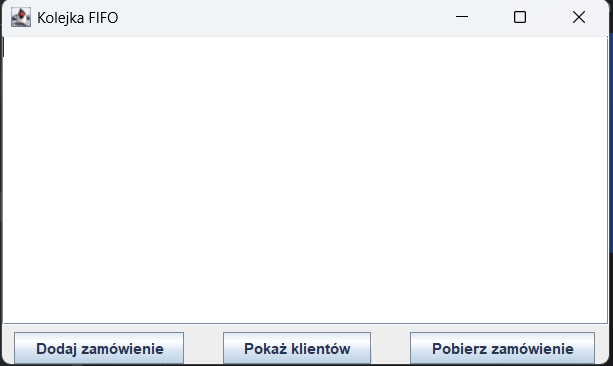
\includegraphics[width=0.7\linewidth]{figures/screenshot001}
	\caption{Okno główne}
	\label{fig:screenshot001}
\end{figure}
 
% ------------------------------------------------------------------------
Dodawanie zamówień:

Aby dodać zamówienie należy, nacisnąć przycisk "Dodaj zamówienie". W następnym kroku podajemy
imię i nazwisko


\begin{figure}[H]
	\centering
	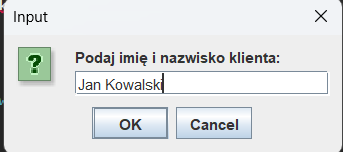
\includegraphics[width=0.7\linewidth]{figures/screenshot002}
	\caption{Podawanie Imiona i nazwiska klienta}
	\label{fig:screenshot002}
\end{figure}
Gdy Klikniemy Ok, program poprosi o wpisanie adresu e-mail.

\begin{figure}[H]
	\centering
	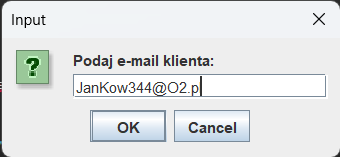
\includegraphics[width=0.7\linewidth]{figures/screenshot003}
	\caption{Wpisywanie Adresu Email}
	\label{fig:screenshot003}
\end{figure}
Po wpisaniu e-maila i wciśnięciu ok, program nas poprosi o wpisanie ilości przedmiotów jaki dany
klient kupił.
\begin{figure}[H]
	\centering
	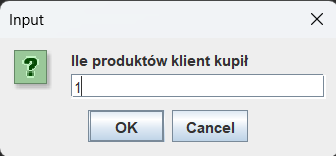
\includegraphics[width=0.7\linewidth]{figures/screenshot004}
	\caption{Podawanie ilości przedmiotów}
	\label{fig:screenshot004}
\end{figure}
Następnie program poprosi o Nazwę produktu, oraz o jego cenę.
\begin{figure}[H]
	\centering
	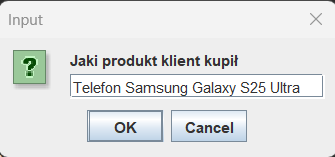
\includegraphics[width=0.7\linewidth]{figures/screenshot005}
	\caption{Podawanie nazwy produktu}
	\label{fig:screenshot005}
\end{figure}
\begin{figure}[H]
	\centering
	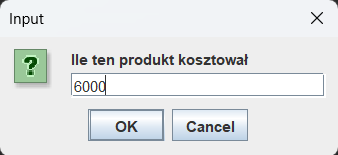
\includegraphics[width=0.7\linewidth]{figures/screenshot006}
	\caption{Podawanie ceny produktu}
	\label{fig:screenshot006}
\end{figure}
Po zakończeniu wszystkich powyższych kroków, program wypisze, dane zamówienia.
\begin{figure}[H]
	\centering
	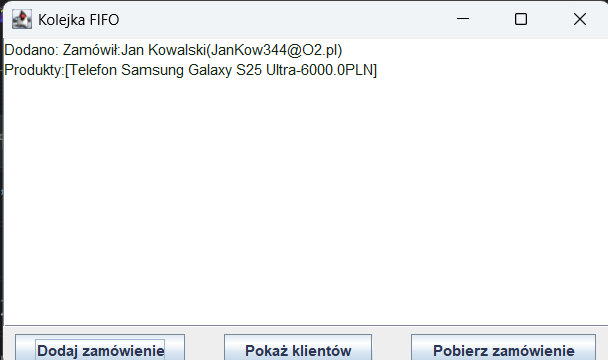
\includegraphics[width=0.7\linewidth]{figures/screenshot007}
	\caption{Wyświetlanie danych dodanego sprzedawcy}
	\label{fig:screenshot007}
\end{figure}


% ------------------------------------------------------------------------
Przetwarzanie zamówień:

Aby przetworzyć zamówienie należy nacisnać przycisk "Pobierz zamówienie". Po przetworzeniu zamówienia
wyświetla się potwierdzenie jego realizacji.
\begin{figure}[H]
	\centering
	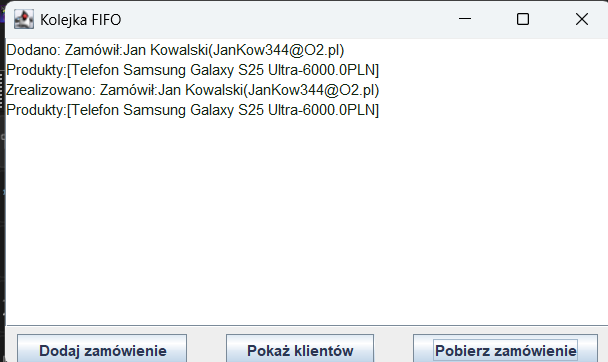
\includegraphics[width=0.7\linewidth]{figures/screenshot008}
	\caption{Realizacja Zamówienia}
	\label{fig:screenshot008}
\end{figure}
W przypadku, próby przetworzenia zamówienia przy pustej kolejce, zostanie wyświetlany napis "Brak
zamówień w kolejce!"
\begin{figure}[H]
	\centering
	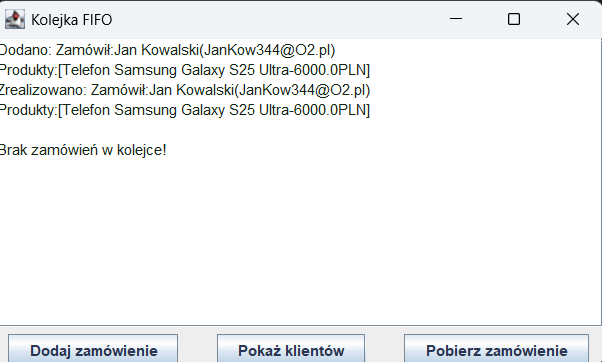
\includegraphics[width=0.7\linewidth]{figures/screenshot009}
	\caption{Próba realizacji zamówienia, gdy kolejka jest pusta}
	\label{fig:screenshot009}
\end{figure}

% ------------------------------------------------------------------------

Naciśnięcie przycisku "pokaż klientów" powoduje wyświetlenie, historii zamówień w bazie danych.
\begin{figure}[H]
	\centering
	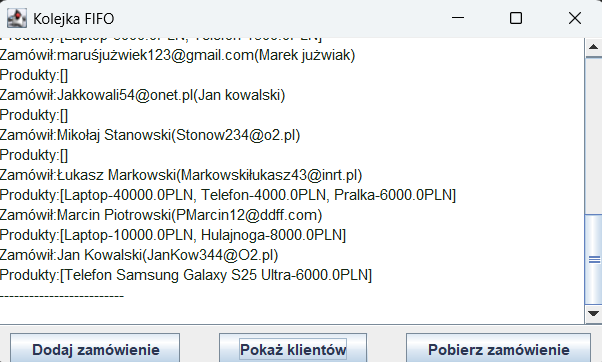
\includegraphics[width=0.7\linewidth]{figures/screenshot010}
	\caption{Wyświetlanie zamówień z bazy danych}
	\label{fig:screenshot010}
\end{figure}


\section{Bazy Danych MySQL}

MySQL to popularny, relacyjny system zarządzania bazami danych, oparty na języku SQL. Jest dostępny jako oprogramowanie open source i rozwijany przez firmę Oracle Corporation. Poniżej znajduje się klasa w języku Java, która odpowiada za połączenie z tą bazą Danych. 
Klasa MenagerBazyDanych:

\lstinputlisting[caption= Klasa MenagerBazyDanych, label=MenagerBazyDanych, style = javaStyle]{src/MenagerBazyDanych.java}


\section{Prezentacja kodu}

Klasa Main (Główna trasa służaca do uruchomienia programu)
\lstinputlisting[style = javaStyle, caption= Klasa Main (główna), label=Main]{src/Main.java}
Klasa GUI (Odpowiedzialna za graficzny interfejs użytkownika)
\lstinputlisting[style = javaStyle, caption= Klasa GUI (Odpowiedzialna za graficzny interfejs użytkownika), label=GUI]{src/GUI.java}
Klasa Klient(Klasa służąca do przechowywania danych klienta)
\lstinputlisting[style = javaStyle, caption= Klasa Klient(Klasa służąca do przechowywania danych klienta), label=Klient]{src/Klient.java}
Klasa Produkt(Klasa służąca do przechowywania informacji o
produkcie)
\lstinputlisting[style = javaStyle, caption= Klasa Produkt(Klasa służąca do przechowywania informacji o produkcie), label=Produkt]{src/Produkt.java}
Klasa Zamówienie
\lstinputlisting[style = javaStyle, caption= Klasa Zamówienia, label=zamowienia]{src/Zamowienie.java}
Klasa KolejkaZamówień
\lstinputlisting[style = javaStyle, caption= Klasa KolejkaZamówień, label=KolejkaZamówień]{src/KolejkaZamowien.java}

% ------------------------------------------------------------------------
\label{key}\chapter{Podsumowanie}
\label{cha:elementyPracyproj}
\section{Podsumowanie ogólne}
Projekt zakładał stworzenie aplikacji desktopowej wspomagającej zarządzanie zamówieniami w kolejce FIFO. Osiągnięto wszystkie założone cele, w tym poprawne działanie kolejki, zapis i odczyt danych z bazy oraz prosty graficzny interfejs.

% ********************
Możliwości rozwoju:
\begin{itemize}
    \item logowanie użytkowników
    \item generowanie faktur PDF
    \item Rozdzielenie bazy danych, przechowującej klientów, produkty oraz Zamówienia.
    \item Pokazywanie ilości produktów w magazynie.
    \item Integrację z systemem wysyłek.
    \item W przypadku braku produktu, na półkach, uniemożliwienie jego zakupu.
\end{itemize}


\section{Harmonogram realizacji projektu}

\begin{figure}[H]
	\centering
	\includegraphics[width=0.7\linewidth]{../../Downloads/diagram_gantta}
	\caption{Harmonogram realizacji projektu}
	\label{fig:diagramgantta}
\end{figure}


\section{Wnioski}

Projekt udowadnia, że przy użyciu podstawowych narzędzi Javy można stworzyć w pełni działający
system do zarządzania zamówieniami, z czytelnym GUI oraz trwałym przechowywaniem danych. Kod jest
modularny, co ułatwia jego dalszy rozwój i integrację z innymi systemami. Istnieje jednak kilka opcji rozwoju programu w kierunku bardziej zaawansowanego narzęcia do zarządzania w bardziej profesjonalny sposób zakupami, stanem magazynu m.in: Przez dodanie stanów magazynów, możliwość logowania, zarówno pracowników jak i klientów.


\section{Oświadczenie studenta o samodzielności pracy}

Oświadczenie należy wydrukować, podpisać, zeskanować i umieścić jako załącznik do niniejszej dokumentacji.

\begin{figure}[H]
	\centering
	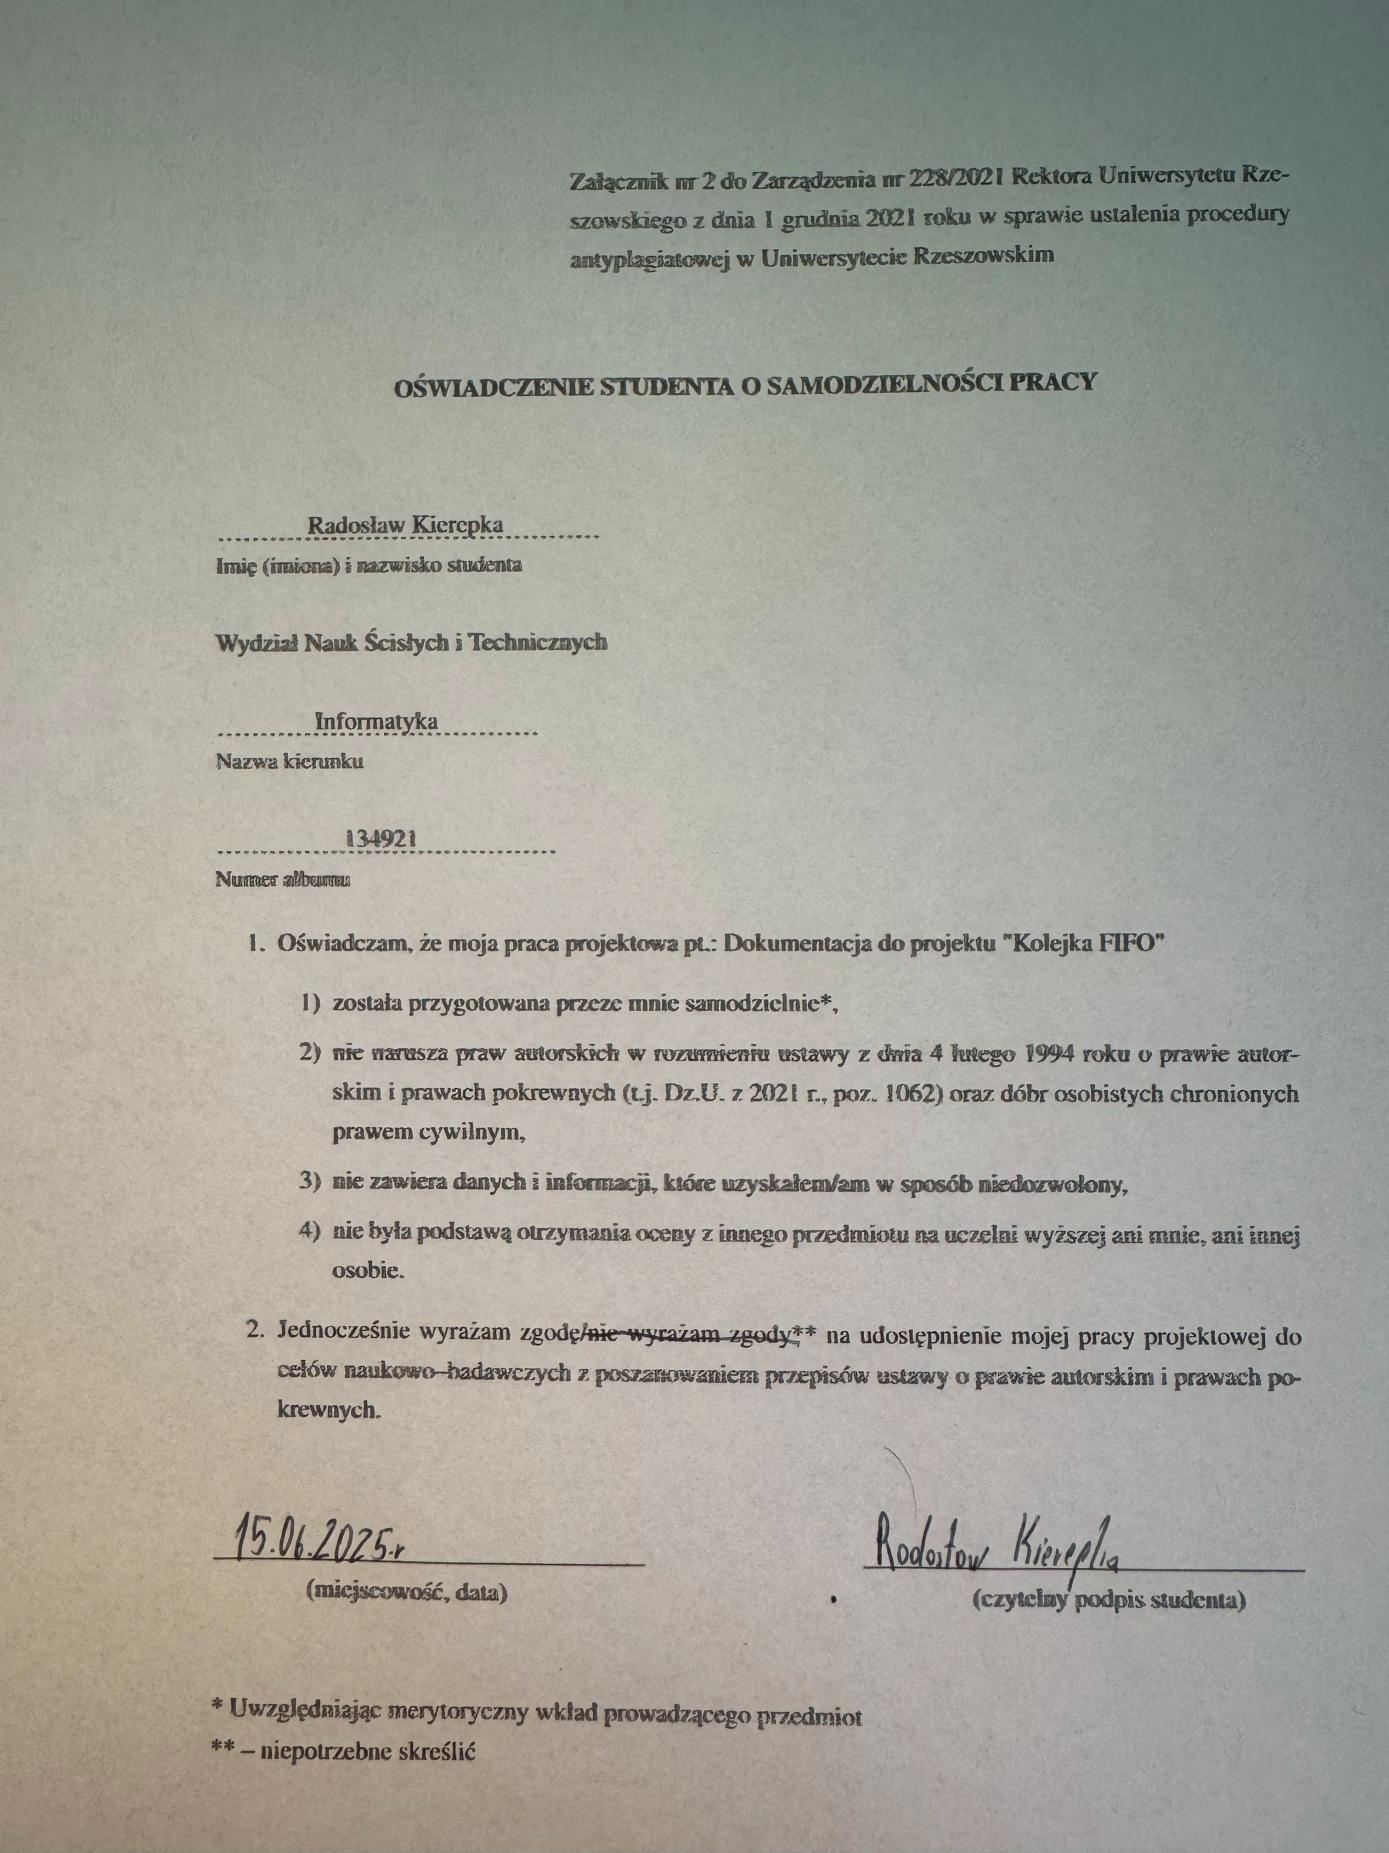
\includegraphics[width=0.7\linewidth]{screenshot001}
	\caption{Oświadczenie studenta o samodzielności pracy}
	\label{fig:screenshot00}
\end{figure}


% ********** Koniec **********

\renewcommand{\emph}[1]{\uline{#1}}
% Bibliografia
% Dodanie bibliografi do spisu treści
\addcontentsline{toc}{section}{\textbf{Bibliografia}}
\bibliographystyle{plain}
\bibliography{bibliografia}

% Przywrócenie działania `ulem`
\renewcommand{\emph}[1]{\uline{#1}}

\clearpage
% Dodanie spisu rysunków do spisu treści
\addcontentsline{toc}{section}{\textbf{Spis rysunków}}
\listoffigures
\clearpage

% Dodanie spisu tabel do spisu treści
\addcontentsline{toc}{section}{\textbf{Spis tabel}}
\listoftables
\clearpage


\clearpage

% Dodanie spisu listingow do spisu treści
\addcontentsline{toc}{section}{\textbf{Spis listingów}}
\lstlistoflistings
\clearpage



\end{document}
